\documentclass[11pt,a4paper]{article}
% \usepackage[utf8]{inputenc}
\usepackage{geometry}
\geometry{a4paper, margin=1in}
\usepackage{graphicx}
\usepackage{booktabs}
\usepackage{hyperref}
\usepackage{titlesec}
\usepackage{xcolor}

% Define a custom color for the headings
\definecolor{techblue}{RGB}{30,58,138}

% Format the section headings
\titleformat{\section}
  {\normalfont\Large\bfseries\color{techblue}}{\thesection}{1em}{}[{\titlerule[0.8pt]}]

\title{\textbf{Research Summary \& Objectives} \\ \large Design of an Authentication Mechanism for ECHONET Lite–Based Smart Home Networks}
\author{Prepared by: Muhammad Suhaib \\ Supervisor: Prof. Dr. Selvakumar Manickam}
\date{} % Leave date empty or add specific date if required

\begin{document}

\maketitle

\section{Introduction \& Problem Statement}
The Internet of Things (IoT) has become a primary driver of digital transformation, with Smart Home Environments (SHEs) standing out as one of the most rapidly expanding IoT deployments. Within these environments, communication protocols are heavily relied upon to facilitate interoperability between consumer electronics, sensors, and energy devices. Echonet Lite serves as a standardized, IP-based application-layer communication protocol specifically designed for smart homes and energy management systems.

Despite its widespread adoption to enable cross-vendor interoperability, Echonet Lite inherently lacks a mandatory built-in authentication mechanism. Consequently, the protocol typically assumes a trusted local network environment or depends on optional external security measures. This absence of standardized freshness verification and authentication directly exposes constrained smart home devices to severe cyber threats, notably replay attacks, Denial of Service (DoS), and Economic Denial of Service (EDoS). Existing security alternatives are often neither lightweight enough nor fully standardized for such resource-constrained endpoints.

\section{Research Objectives}
To address the critical security vulnerabilities in the current Echonet Lite protocol, this research proposes the following primary objectives:
\begin{itemize}
    \item To propose a robust authentication mechanism for Echonet Lite that minimizes the reliance on optional external security layers, ensuring it remains highly suitable for constrained smart home devices.
    \item  To formulate cryptographic protections specifically tailored for Echonet Lite capable of mitigating replay, DoS, and EDoS attacks while maintaining minimal performance overhead.
\end{itemize}

\section{Methodology \& Experimental Scope}
The research is heavily design-oriented and experimental, structured into four strategic phases:
\begin{itemize}
    \item \textbf{Phase 1:} Identification of absent security features, focusing specifically on authentication and message freshness, alongside a structural analysis of the Echonet Lite protocol flow and object model.
    \item \textbf{Phase 2:} Development of a protocol-level authentication scheme, introducing a Security Extension Field (SEF) that maintains backward compatibility with the existing framework.
    \item \textbf{Phase 3:} Implementation of the proposed mechanism within a simulated Echonet Lite environment, modeling both the controller and end-device communication behaviors.
    \item \textbf{Phase 4:} Quantitative evaluation measuring the communication and processing overhead introduced by the new authentication fields, comparing the standard protocol against the newly authenticated variant.
\end{itemize}

The scope targets the Application Layer within a UDP/IP network environment. Evaluation metrics are strictly focused on processing time, control overhead, and the attack prevention success rate against DoS, replay, and EDoS attacks.

\begin{figure}[htbp]
    \centering
    % Assuming the image is in the same directory as the .tex file
    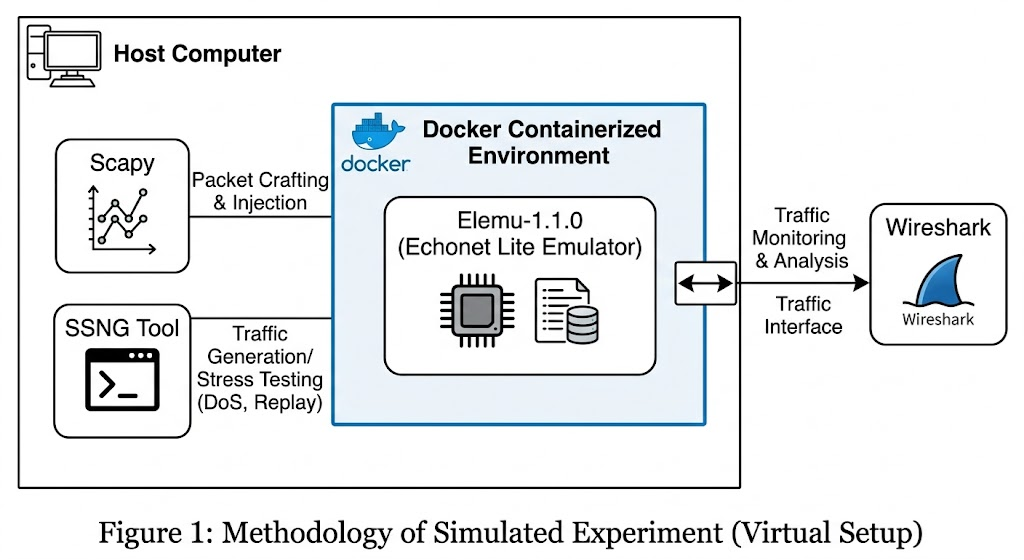
\includegraphics[width=0.8\textwidth]{assets/Experiment 1.png}
    \caption{Methodology of Simulated Experiment (Virtual Setup) utilizing Elemu-1.1.0, Docker, and Scapy for traffic generation and analysis.}
    \label{fig:assets/Experiment 1.png}
\end{figure}

\begin{figure}[htbp]
    \centering
    % Assuming the image is in the same directory as the .tex file
    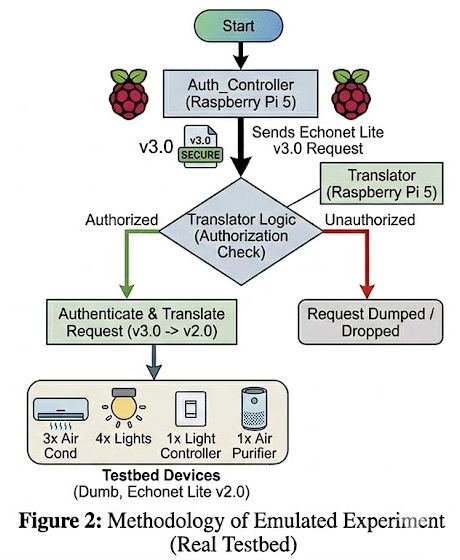
\includegraphics[width=0.6\textwidth]{assets/Experiment 2-Testbed Setup.png}
    \caption{Methodology of Emulated Experiment on a Real Testbed using Raspberry Pi controllers and physical smart home devices.}
    \label{fig:assets/Experiment 2-Testbed Setup.png}
\end{figure}

\section{Preliminary Findings \& Expected Outcomes}
Initial implementation milestones successfully validated four distinct secure communication models for ECHONET-Lite environments. The quantitative analysis highlights the critical trade-offs between enhanced security and transmission overhead.

\begin{table}[htbp]
    \centering
    \caption{Packet Size and Security Overhead Analysis}
    \begin{tabular}{lccc}
        \toprule
        \textbf{Security Model} & \textbf{Avg. Total Size (B)} & \textbf{Avg. Payload (B)} & \textbf{Avg. Security Overhead (B)} \\
        \midrule
        NATIVE (Baseline) & 20.40 & 20.40 & 0.00 \\
        \textbf{ELAF (Proposed)} & \textbf{44.72} & \textbf{21.72} & \textbf{23.00} \\
        DTLS (Standard) & 62.89 & 17.89 & 45.00 \\
        JWT (Token-based) & 148.40 & 20.40 & 128.00 \\
        \bottomrule
    \end{tabular}
\end{table}

\vspace{0.5cm}
\noindent\textbf{Core Technical Contributions:}
\begin{itemize}
    \item \textbf{Efficiency:} The proposed ECHONET Lite Authentication Framework (ELAF) is confirmed as the most efficient secure alternative. By introducing a Security Extension Field containing timestamps, counters, and HMACs, it adds merely 23 bytes of overhead per packet, drastically outperforming JWT (128B overhead).
    \item \textbf{Attack Resilience:} The integration of authentication on critical packet fields enables the immediate rejection of spoofed/malformed packets (mitigating DoS) and prevents unnecessary cryptographic processing, thereby protecting device battery and processing limits (mitigating EDoS). Monotonic counters and timestamps effectively detect and discard stale or maliciously replayed packets.
\end{itemize}

\end{document}
